% Класс документов по ГОСТ 7.32-2001 "Отчёт о научно-исследовательской работе"
% на основе ГОСТ 2.105-95
% Автор - Алексей Томин, с помощью списка рассылки latex-gost-request@ice.ru,
%  "extreport.cls", "lastpage.sty" и конференции RU.TEX
% Лицензия GPL
% Все вопросы, замечания и пожелания сюда: mailto:alxt@yandex.ru
% Дальнейшая разработка и поддержка - Михаил Конник,
% связаться можно по адресу mydebianblog@gmail.com

\documentclass[utf8,usehyperref,12pt]{G7-32}
\usepackage[T2A]{fontenc}
\usepackage[utf8]{inputenc} %% ваша любимая кодировка здесь
\usepackage[english,russian]{babel} %% это необходимо для включения переносов
\usepackage{float}
\usepackage{graphicx}
\graphicspath{{pictures/}}

\TableInChaper % таблицы будут нумероваться в пределах раздела
\PicInChaper   % рисунки будут нумероваться в пределах раздела
\setlength\GostItemGap{2mm}% для красоты можно менять от 0мм

% Определяем заголовки для титульной страницы
\NirOrgLongName{\textsc{НАЦИОНАЛЬНЫЙ ИССЛЕДОВАТЕЛЬСКИЙ ЯДЕРНЫЙ УНИВЕРСИТЕТ «МИФИ» }} %% Полное название организации

\NirBoss{Директор ООО <<Рога и Копыта>>}{И.И.Иванов} %% Заказчик, утверждающий НИР
\NirManager{инженер}{Д.Е. Катаев} %% Название организации

\NirYear{2013}%% если нужно помен\label{?} ять год отчёта; если закомментировано, ставится текущий год
\NirTown{г. Москва,} %% город, в котором написан отчёт
% по проекту \No8550: 

% \NirIsAnnotacion{АННОТАЦИОННЫЙ } %% Раскомментируйте, если это аннотационный отчёт

\NirUdk{УДК \No 2123132123}
\NirGosNo{Регистрационный \No 123123}

\NirStage{Этап \No 1.1}{промежуточный}{<<Обзор современного состояния торсионных наногенераторов>>} %%% Этап НИР: {номер этапа}{вид отчёта - промежуточный или заключительный}{название этапа}

\bibliographystyle{unsrt} %Стиль библиографических ссылок БибТеХа

%%%%%%%<------------- НАЧАЛО ДОКУМЕНТА
\begin{document}
\usefont{T2A}{ftm}{m}{} %%% Использование шрифтов Т2 для возможности скопировать текст из PDF-файлов.

\frontmatter %%% <-- это выключает нумерацию ВСЕГО; здесь начинаются ненумерованные главы типа Исполнители, Обозначения и прочее

\NirTitle{\textbf{«Оптимизация обучающих выборок с помощью генетического алгоритма»}} %%% Название НИР и генерация титульного листа«»


\Executors %% Список исполнителей здесь
%% это рисует линию размера 3мм и толщиной 0.1 пункт
\begin{longtable}{p{0.35\linewidth}p{0.2\linewidth}p{0.35\linewidth}}
Научный руководитель, 	&		&	\\
доцент К.К.Петров	&\rule{1\linewidth}{0.1pt}	&  \\ \vspace{1cm}

с.н.с, к.т.н,  &		&	\\
Ж.Ж. Балбесов, & \rule{1\linewidth}{0.1pt}& \\
\end{longtable}
\Referat
 Отчет \totalpages~с, \totaltables~таблица, \totalfigures~рисунок, \totalbibs~источник.
\tableofcontents

\Introduction
Одним из ключевых моментов в реализации систем, использующих алгоритмы машинного обучения с учителем является подготовка обучающей выборки. В настоящее время, как правило, синтез обучающей выборки выполняется экспертом.ъ, который, однако, далеко не для всех задач в состоянии за разумное время выбрать и представить исходные данные задачи в оптимальном для обучаемой системы виде. Таким образмо имеется потребонсть в системах, которые способны автоматически формировать обучающие выборки для интеллектуальных систем из имеющихся данных таким образом, чтобы их обучение по автоматически сформированным выборкам было максимально эффективным. Естественно, подобные системы востребованы только в тез случаях, когда либо не существует, либо не сформулирован алгоритм формирования обучающей выборки. Таким образом наиболее иодходящим выглядит использование алгоритмов случайного поиска, например генетических.

Цель данной работы разработка новой версии ПО для генетической оптимизации обучющих выборок систем машинного обучения с учителем. Модификация алгоритма для устранения избыточности обучающих данных. А так же оценка класса решаемых алгоритмом задач.

\mainmatter %% это включает нумерацию глав и секций в документе ниже
\chapter{Постановка задачи}
Основной задачей являлась разработка новой версии программного обеспечения для оптимизации обучающих выборок при помощи генетического алгоритма на основе старой с реализацией ряда модификаций:
\begin{enumerate}
\item Модификация формата вывода данных для облегчения взаимодействия с пользователем
\item Устранение избыточности обучающих данных для снижения вычислительной мощности
\item Модификация алгоритма мутации для реализации рекурсивной мутации 
%\item Реализация на Python
\end{enumerate}	
\section{Описание исходной системы}
Пусть $ f(S_{h})=(S_{t}; S_{v})) $ - отображение $f$ исторических данных $S_{h}$ в совокупность обучающей $S_{t}$ и валидационной $S_{v}$ выборок. Пусть $ N(S_{t}; S_{v}) $ - искусственная нейронная сеть прямого распространения, обученная по $S_{t}$ и проверяемая по $S_{v}$, а $ Err_{v}(N(S_{t}; S_{v})) $ - ее ошибка валидации, определяемая, как среднеквадратичное отклонение всех выходов сети от соответствующих эталонных значений при подаче на вход элементов валидационной выборки. Тогда
\begin{equation}
\exists\bar{f}:\bar{f}(S_{h})=arg\{min Err_{v}(N(S_{t}; S_{v})). \}
\end{equation}
Требуется найти $ \bar{f} $. Для этого реализован следующий алгоритм, представленный на рис. ~\ref{algo} \\
Критерием останова в используемой реализации является прохождение заданного количества итераций. В текущей реализации используются ИНС прямого распространения в одним скрытым слоем, обучаемые методов эластичного распространения (RPROP)\\
Отображения $f$ представляют собой конструкции следующего вида:
\begin{equation}
f(S_{h})=\begin{array}{|c|}
(\lambda_{i_{1}} \circ \lambda_{i_{2}} \circ ... \circ \lambda_{i_{m}})(S_{h_{j_{1}}}) \\
...\\
(\lambda_{i_{n-l}} \circ ... \circ \lambda_{i_{n}})(S_{h_{j_{k}}})
\end{array}
, \lambda\in\Lambda, i,n,m,j\in N,
\end{equation}
где $\Lambda$ - множество доступных системе элементарных преобразований сигналов (дифференцирование, фильтры, добавление лагов и т.п.), $S_{h_{j}}$ - произвольный сигнал из исторических данных. Атомарной единицей при кроссовере является $f(S_{h})_{i}$, однако мутации возможны и внутри нее.\\
\begin{figure}[H]
 \caption{Схема используемого алгоритма}\label{algo}
 \centering{
 	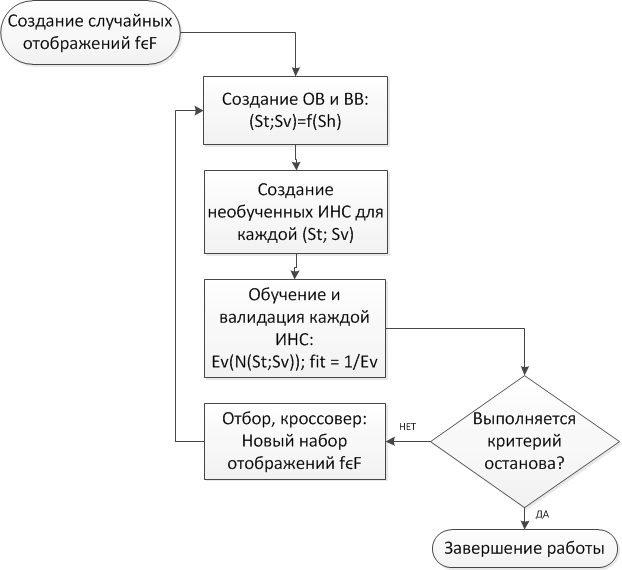
\includegraphics[width=0.4\textwidth]{algo.png}
  }
\end{figure}

При хранении экземпляр кодировался линейной последовательностью исполняемых команд и списком команд, результаты выполенения которых попадают в обучающую выборку. Такая структура данных не способствовала тонкой настройке алгоритмов кроссовера и мутации.
\section{описание стоящих задач}
\subsection{Модификация структуры вывода данных}
В силу тяжести взаимодействия пользователь с исходным форматом вывода данных было решено сменить формат вывода данных. Целями смены формата были: повышение человекочитаемости, повышение легкости транспортировки и модифицирования данных эксперимента,по возможности сохранение легкости загрузки данных в приложение.
Возможными структурами хранения при решении данной задачи были xml, json, исполняемый код или база данных. К плюсам xml при решении поставленной задачи следует отнести следующее:
\begin{longtable}{|c|p{0.25\linewidth}|p{0.25\linewidth}|p{0.25\linewidth}|}
\multicolumn{4}{l}{\tablename asd\label{T:Ta}}\\
\hline
Средство & Читаемость & Транспортабельность & Скорость \\
\hline
\endfirsthead
\multicolumn{4}{l}{Продолжение таблицы~\ref{T:Ta}}\\
\hline
Средство & Читаемость & Транспортабельность & Скорость \\
\hline
\endhead
XML & Читаемый в сыром виде формат. Для прочтения в удобном виде достаточно элементарного браузера & Для передачи достаточно просто переслать интересующее поддерево, или целиком файл. & Париснг требует затрат времени. Затраты, однако, можно сократить оптимизацией, основанной на жесткости структуры.   \\
JSON & Читаемость формата в сыром виде несколько затруднена. Требуется специальный просмотровщик. & Для передачи достаточно переслать интересующий объект, или целиком файл. & Парсинг требует минимального времени - фактически это преобразование из строки в код. \\
Исполняемый код & Читаемость формата в сыром виде требует специальных навыков. Желательна подсветка синтаксиса и знание структуры программы. & Для передачи данных достаточно передать цельный кусок кода, что однако тоже требует специальных навыков. & Парсинг требует минимального времени - фактически это преобразование из строки в исполняемый код. \\
База данных &
Читаемость в сыром виде практически отсутствует как класс. Требуются специальные просмотровщики. Цельность данных с точки зрения просмотра теряется. &
Передача данных как таковых требует либо объединенной БД для нескльких экземпляров системы, между которыми идет передача, либо выгрузки из базы данных &
Скорость работы зависит от СУБД и скорости соединения, если база данных удалена, однако скорость работы любой базы данных на локальной машине - выше, чем скорость преобразования текстовых файлов. \\
\hline
\end{longtable}
По результатам выбора между представленными альтернативами был выбран формат данных xml.

\subsection{Устранение избыточности обучающих данных}
В предыдущей версии возникла проблема избыточности размера экземпляров, которая достаточно критично влияла на объем  вычислений, производимых системой. Задачей является сокращение роста экземпляров, при сохранении возможности такого роста.

Устранить избыточность обучающих данных можно было при помощи нескольких модификаций:
\begin{enumerate}
\item Выкидывание на каждой мутационной фазе алгоритма одного элемента из экземпляра и проверка направления изменения фитнесс-функции
\item Жесткое ограничение на размер экземпляра
\item Изменения распределения вероятностей в пользу уменьшения, а не увеличения размера экземпляра
\end{enumerate}
Вариант с жестким ограничением на размер экземпляра был отвергнут в связи с невозможностью в общем случае предугадать рельную правильную длину. Вариант с изменением алгоритма мутации был исключен в силу увеличения времени работы каждого шага почти в два раза. Реализуемым вариантом стал вариант с изменением распределения вероятностей. Конкретным изменением послужило увеличение возможного интервала размеров на следующем шаге в сторону уменьшения.

\subsection{Модификация алгоритма мутации для реализации рекурсивной мутации}
Для осуществления возможности вносить большее разнообразие в экземпляры и большей настраивамости хода работы алгоритма требовалось введение возможности мутировать не только атомарные объекты но и структуры их объединяющие.

Для реализации рекурсивной мутации в каждой сущности, вплоть до атомарного элемента - функции ЦОС, была модифицирована процедура мутации. На фазе мутации каждая сущность верхнего уровня с заданной вероятностью мутировала полностью - генерировался полностью новый экземпляр этой сущности, в обратном же случае она вызывала мутацию всех своих сущностей-детей.

%\subsection{Реализация на Python}	
%В ходе разработки новой версии возникла потребность реализовать систему набором средств предоставляющих инструментарий для легкой поддержки и модификации системы.
%
%В качестве языка разработки был выбран python версии 2.7. python на данный момент является широко распространенным языком для научной разработки. Набор библиотек позволяет не заниматься реализацией большинства общепринятых алгоритмов, например алгоритм обучения с учителем. Язык обладает четким и последовательным синтаксисом, а так же хорошей масштабируемостью, что позволяет сохранить читаемость, сопровождаемость и дополняемость кода. К тому же Python умеет работать с такими языками как Fortran, C и С++, которые уже широко используются в научных расчетах.

\chapter{Описание программного обеспечения}
Текущая версия ПО представляет из себя пакет скриптов на языке python версии 2.7, содержащий инструменты для проведения вычислений и анализа результатов.

Алгоритм по существу не менялся по сравнению с прошлой версией. Однако изменению подверглись его подалгоритмы и методы реализации.

Модуль вычислений описан в диаграмме классов \ref{class-diagram}
\begin{figure}[H]
 \caption{диаграмма классов модуля проведения вычислений}\label{class-diagram}
 \centering{
 	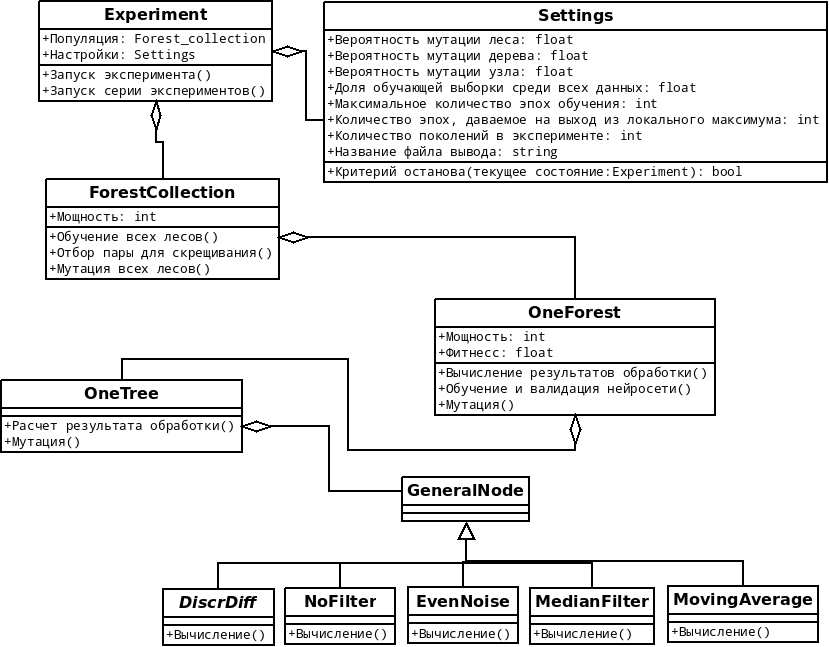
\includegraphics[width=0.9\textwidth]{class-diagram.png}
  }
\end{figure}
Для инициализации вычислений требуется представить входные данные для обработки и входные данные для вычислительного модуля. Стандартным методом получения данных для обработки является набор csv файлов со значениями. Входные данные для вычислительного модуля фактически представляют из себя экземпляр класса настроек. Выходные данные вычислительного модуля представлены в XML формате, и выгружаются в файл с настраиваемым названием.

Модуль обработки результатов вычислений представляет из себя набор скриптов, позволяющих собирать информацию о ходе и результатах генетического алгоритма как с одного, так и с набора XML файлов. По результатам работы строит csv файл содержащий в себе выбранные и обработанные значения.
 
Используемые библиотеки:
PyBrain - для создания и обучения искуственных нейросетей.
SciPy и NumPy - для ускорения вычислений.

\chapter{Эксперименты}
\section{Используемые тестовые сценарии}
Для тестирования использовалось два типа систем - линейная и нелинейная. Под сценарием эксперимента подразумевается набор из входных и целевых данных для нейросети.
\subsection{Линейная система}
Пусть существует бассейн, который является объектом управления. К нему подведены две трубы: через одну в бассейн может поступать вода с произвольной скоростью (в данном тестовом сценарии не будут учитываться физические ограничения), через вторую трубу вода может уходить из бассейна с произвольной скоростью. Через эти две трубы осуществляется управление бассейном. Ограничения на то, что объем воды в бассейне должен быть неотрицательным нет, но, стоит отметить, что в данном сценарии не возникает соответствующей ситуации.\\
Пусть существуют следующие экспериментальные данные:\\
$ X^{(0)} $ – объем поступившей за $ \Delta t $ воды;\\
$ X^{(1)} $ – объем откачанной за $ \Delta t $ воды;\\
$ X^{(2)} $ – объем воды, находящейся в бассейне в данный момент времени;\\
$ X^{(3)} $ – посторонний сигнал, отличающийся от остальных;\\
Реально бассейн реагирует на управляющие воздействия следующим образом:\\
\begin{equation}
X^{(2)}_{i} = X^{(2)}_{i-1} + X^{(0)}_{i-1} - X^{(1)}_{i-1}; X^{(2)}_{0}=10
\end{equation}


Пусть испытуемая система не имеет априорной информации об объекте управления и имеет доступ к следующим данным в качестве исходных:\\
$ X^{(0) \Delta t} $ – объем поступившей за $ \Delta t $ воды, на этот сигнал наложен импульсный шум (inflow\_noizd);\\
$ X^{(1) \Delta t} $ – объем откачанной за $ \Delta t $ воды (outflow);\\
$ X^{(3)} $ – посторонний сигнал (trash).\\
\subsection{Нелинейная система}
Пусть $ X^{(0)}, .., X^{(5)}$ – действительные временные ряды\\
из которых $ X^{(3)}, .., X^{(5)}$ не оказывают на систему никакого реального воздействия.\\
$ X^{(6)} $ - выход системы\\
Реально система реагирует на управляющие воздействия следующим образом:\\
\begin{equation}
X^{(6)}_{i} = |X^{(0)} - X^{(1)}| + X^{(2)};
\end{equation}
Перед подачей в вычислительный модуль на $ X^{(0)} $ был наложен постоянный шум с амплитудой 0.5, на $ X^{(1)} $ наложен шум с вероятностью 2.5\% прибавляющий 1 и с такой же - вычитающей (условно такой шум можно считать импульсным). Остальные сигналы зашумлению не подвергались.

\section{Устранение избыточности}
В качестве эксперимента для проверки работоспособности решения по устранению избыточности было решено провести пару тестов на одинаковых входных данных для старого и нового алгоритмов кроссовера. В качестве метрики для сравнения был выбран размер экземпляра на определенной итерации, усредненный среди нескольких экспериментов, для устранения возможности влияния случайных факторов.
\begin{figure}[H]
 \caption{график средних размеров экземпляров по поколениям для старого и нового алгоритма}\label{cross_diff}
 \centering{
 	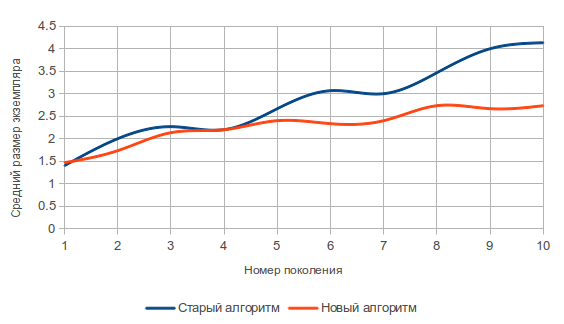
\includegraphics[width=0.6\textwidth]{crossover_difference.png}
  }
\end{figure}
Средняя производная по таким графикам различается в два раза в пользу новой версии алгоритма кроссовера, что говорит о решении данной поставленной задачи по крайней мере в ограниченном объеме.

\section{Модернизация алгоритма мутации}
Для оценки качества модификации алгоритма мутации было проведено равное количество экспериментов при одинаковых начальных условиях для старого и нового алгоритма мутации, для разных вероятностей мутации. Для моделирования старого алгоритма (Плоский случай) новому задавались нулевыми вероятности мутации всех элементов кроме атомарных - функций ЦОС. Для моделирования аналогичной вероятности с использованием рекурсивной мутации вероятности выставлялись одинаковыми и равными приведенной вероятности рассчитаной по формуле. \ref{equiv_prob}
\begin{equation}
P_{n}=\sqrt[3]{p-1}+1
\label{equiv_prob}
\end{equation}
Где $ p $ - вероятность для плоского случая (приведенная вероятность), а $ P_{n} $ - аналогичная ей вероятность для рекурсивного случая.

На основе экспериментов проведенных с линейной системой построены графики приведенные на рисунках \ref{mutate_diff_fit} и \ref{mutate_diff_gen}. На основе графика  \ref{mutate_diff_gen} можно сказать, что после реализации новой версии мутации уменьшилось время сходимости алгоритма, а так как на графике \ref{mutate_diff_fit} видно, что фитнесс-функция оптимального экземпляра не только не ухудшилась но и улучшилась при таком переходе, можно сказать что мы не столкнулись с явлением преждевременной сходимости.
\begin{figure}[H]
 \caption{средняя фитнесс-функция для приведенных вероятностей мутации}\label{mutate_diff_fit}
 \centering{
 	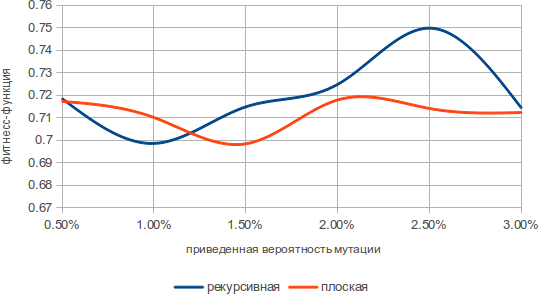
\includegraphics[width=0.6\textwidth]{mutation_difference_fit.png}
  }
\end{figure}
\begin{figure}[H]
 \caption{время сходимости для приведенных вероятностей мутации}\label{mutate_diff_gen}
 \centering{
 	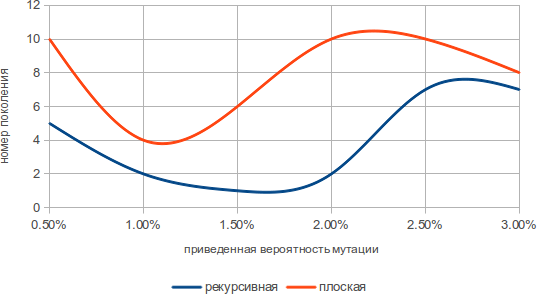
\includegraphics[width=0.6\textwidth]{mutation_difference_gen.png}
  }
\end{figure}


На основе экспериментов проведенных с нелинейной системой построены графики приведенные на рисунках \ref{mutate_diff_fit_nl} и \ref{mutate_diff_gen_nl}. Среднее значение на графике \ref{mutate_diff_fit_nl} для рекурсивной мутации превышает среднее значение для плоской. То есть в целом рекурсивная мутация сходится к более высокому значению. Как видно на графике \ref{mutate_diff_gen_nl} рекурсивный алгоритм почти всегда сходится быстрее, а так же сходится быстрее в среднем.
\begin{figure}[H]
 \caption{средняя фитнесс-функция для приведенных вероятностей мутации}\label{mutate_diff_fit_nl}
 \centering{
 	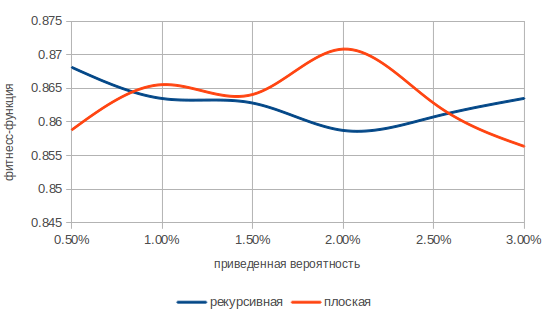
\includegraphics[width=0.625\textwidth]{mutation_difference_fit_nl.png}
  }
\end{figure}
\begin{figure}[H]
 \caption{время сходимости для приведенных вероятностей мутации}\label{mutate_diff_gen_nl}
 \centering{
 	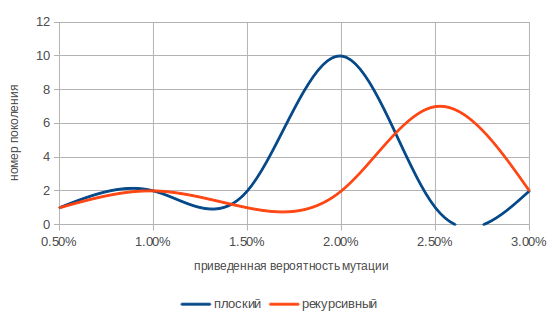
\includegraphics[width=0.625\textwidth]{mutation_difference_gen_nl.png}
  }
\end{figure}


%В качестве средств повышения сопровождаемости кода были выбраны:
%\begin{enumerate}
%\item Смена языка разработки на язык ориентированный на прозрачность исходного кода
%\item Следование рекомендациям PEP8 и PEP257 для разработчиков на языке Python, что приводило код и комментарии к нему к монотипно читаемому виду.
%\item Работа с git в качестве системы контроля версий, что позволяет отследить историю изменений в коде
%\item хранение хода и результатов каждого отдельного эксперимента в виде xml что позволяет провести анализ не только результатов набора экспериментов но и анализ отдельных деталей вплоть до просмотра конкретной хромосомы конкретного экземпляра конкретного поколения в конкретном эксперименте 
%\end{enumerate}

В качестве оценок качества кода и сопровождаемости были выбраны следующие эксперименты, метрики и критерии:
\begin{enumerate}
\item Валидация PEP8 \& PEP257
\item Проведение ряда экспериментов работавших в прошлой версии ПО, как средство проверки правильности практической реализации алгоритма
\item Сравнение характеристик сходимости при старом и новом алгоритме мутации
\end{enumerate}

\section{Модификация структуры вывода данных}
В силу вычислительной сложности задачи эксперименты зачастую ставились на сторонней машине, после чего результаты вычислений пересылались для анализа на основную машину. Путь передачи с копированием XML файлов показал себя как надежный и простой. За время передачи данных не произошло ни одной потери и синхронная включенность обеих машин не требовалась для передачи данных.



В отчётах могут быть и таблицы - см.табл.~\ref{T:T1}.

\begin{longtable}{|c|c|c|p{110mm}|}
 \multicolumn{4}{l}{\tablename~\thetable~---~Пример таблицы\label{T:T1}}\\\hline
 Название 1  & Название 2 & Название 31 \\
\hline
\endfirsthead
 \multicolumn{4}{l}{Продолжение таблицы~\ref{T:T1}}\\
\hline
1 & 2 & 3 \\
\hline
\endhead
Это  & пример & данных  \\
\hline
помещённых & внутрь & таблицы \\
\hline
\end{longtable}


\backmatter %% Здесь заканчивается нумерованная часть документа и начинаютяс заключение и ссылки

\Conclusion % заключение к отчёту

\begin{thebibliography}{1} %% здесь библиографический список

\bibitem{filosofyNewestdict}
{Грицанов} А.А.~и др.
\newblock {\em Новейший философский словарь}.
\newblock Мн.: Книжный Дом., 2003.

\end{thebibliography}

% \bibliography{biblio/filosofy} %% вместо вставки библиографии можно использовать базы BiBTeX - просто раскомментируйте эту строку.
\end{document}
